\chapter{Einleitung}
\pagenumbering{arabic}

Nach einem langen Spaziergang durch die Innenstadt von K�ln steht eine
Touristin vor dem Dom und m�chte mit den �ffentlichen Verkehrsmitteln wieder
zur�ck in ihr Hotel. Sie greift zum Mobiltelefon und stellt eine Verbindung
zum WAP-Portal ihres Mobilfunkanbieters her. Nach der Auswahl des Men�punktes
{\em �ffentliche Verkehrsmittel} �ffnet sich eine Eingabemaske, in dem
sie ihr Ziel, den Namen ihres Hotels, eingibt. Kurze Zeit sp�ter wird eine
Wegbeschreibung zur n�chstgelegenen Bushaltestelle sowie die Fahrverbindung
zu ihrem Hotel auf dem Display angezeigt.

Insgesamt realisiert das entworfene Szenario einen standortbezogenen Dienst
(Location Based Service). Unter Ausnutzung der Ortbarkeit eines eingeschalteten
Mobiltelefons lassen sich auf die momentane Position abgestimmte Dienste
und Informationen anbieten. F�r die Realisierung eines solchen Szenarios ist
ein Zusammenf�hren verschiedenster Datenquellen erforderlich.

\bigskip

\begin{figure}[htbp]
  \centering
  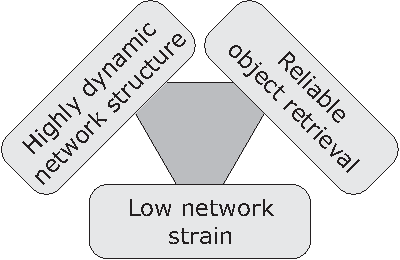
\includegraphics{picture/tradeoff}
  \caption{Tradeoffs in P2P systems}
  \label{fig:tradeoff}
\end{figure}

So beginnt zum Beispiel eine Studienarbeit. Nicht vergessen, hier in der Einleitung auch einen �berblick �ber die einzelnen Kapitel der Arbeit sowie deren Inhalt zu geben! So kann man z.B. mittels \texttt{ref} auf Verweise innerhalb des Dokumentes verweisen, wenn diese mit \texttt{label} vorher definiert wurden. Hier zum Beispiel ein Verweis auf das erste Kapitel im Anhang \ref{app:c1:s1} oder hier einer auf das nun folgende Bild \ref{fig:tradeoff}.

Ganz wichtig sind nat�rlich auch Zitate. Nat�rlich wird daf�r BibTeX verwendet, doch was man daf�r wissen muss, beschr�nkt sich auf relativ wenig: Anlegen und Pflegen einer .bib - Datei, am besten mit dem sehr guten Tool JabRef und zitieren im Text mit \texttt{cite}. So kann man dann beweisen, dass sich in einem Artikel \cite{Herschel2003} �ber Goya ge�u�ert wurde.
